\PassOptionsToPackage{hyphens}{url}
\documentclass{PPFIT} % pro psaní v angličtině / for writing in English
% \documentclass[czech]{PPFIT} % pro psaní v češtině / for writing in Czech
%\documentclass[slovak]{PPFIT} % pro psaní ve slovenštině / for writing in Slovak

\usepackage{pdfpages} % for appending the standalone formalism PDF as Appendix A
\usepackage{xurl}

%--------------------------------------------------------
%--------------------------------------------------------
%	PŘIZPŮSOBENÍ PDF / PDF CUSTOMIZATION
%--------------------------------------------------------

\hypersetup{
	pdftitle={Paper Title},
	pdfauthor={Author},
	pdfkeywords={Keyword1, Keyword2, Keyword3}
}

%--------------------------------------------------------
%--------------------------------------------------------
%  PŘEDBĚŽNÁ vs. KONEČNÁ VERZE / REVIEW vs. FINAL VERSION
%--------------------------------------------------------
%   NECHTE následující řádek zakomentovaný pro PŘEDBĚŽNÉ VERZE
%   Pro KONEČNOU VERZI řádek odkomentujte.
%   LEAVE this line commented out for the REVIEW VERSIONS
%   UNCOMMENT this line to get the FINAL VERSION

%\PPFinalCopy


\PPYear{2025/2026}

\ifczechslovak%
    %--------------------------------------------------------
    %--------------------------------------------------------
    %	INFORMACE O ČLÁNKU
    %--------------------------------------------------------    

  \PaperTitle{Jak napsat skvělý článek}

	\Authors{Adam Herout*}
	\affiliation{*%
	  \href{mailto:herout@fit.vut.cz}{herout@fit.vut.cz},
	  \textit{Fakulta informačních technologií, Vysoké učení technické v Brně}}

	\Keywords{Klíčové slovo1 --- Klíčové slovo2 --- Klíčové slovo3}

	\Supplementary{\href{http://youtu.be/S3msCdn3fNM}{Demonstrační Video} --- \href{http://fit.vut.cz/}{Stáhnutelný Kód}}

    %--------------------------------------------------------
    %--------------------------------------------------------
    %	ABSTRAKT
    %--------------------------------------------------------
    \Abstract{
        O jaký problém se jedná? O jaké téma? Jaký je cíl této práce?
        \phony{Lorem ipsum dolor sit amet, consectetur adipiscing elit. Fusce ullamcorper suscipit euismod. Mauris sed lectus non massa molestie congue. In hac habitasse platea dictumst.}
        %	
        Jak se tento problém řeší a jak je cíle dosaženo (metodika)?
        \phony{Lorem ipsum dolor sit amet, consectetur adipiscing elit. Fusce ullamcorper suscipit euismod. Mauris sed lectus non massa molestie congue. In hac habitasse platea dictumst. Curabitur massa neque, commodo posuere fringilla ut, cursus at dui. Nulla quis purus a justo pellentesque.}
        %	
        Jaké jsou konkrétní výsledky? Jak dobře se daný problém řeší?
        \phony{Lorem ipsum dolor sit amet, consectetur adipiscing elit. Fusce ullamcorper suscipit euismod. Mauris sed lectus non massa molestie congue. In hac habitasse platea dictumst.}
        %	
        Takže co? Jak užitečná je tato práce pro vědu a pro čtenáře?
        \phony{Lorem ipsum dolor sit amet, consectetur adipiscing elit. Fusce ullamcorper suscipit euismod.}
    }
\else%
    %--------------------------------------------------------
    %--------------------------------------------------------
    %	INFORMATION ABOUT THE ARTICLE
    %--------------------------------------------------------
    \PaperTitle{Evaluating Test Completeness Against Software Requirements}

	\Authors{Bc. Jakub Bláha}
	\affiliation{*%
		\href{mailto:xblaha36@vutbr.cz}{xblaha36@vutbr.cz},
		\textit{Faculty of Information Technology, Brno University of Technology}}

	\Keywords{NL-to-formal translation --- requirements formalisation --- test coverage gap detection --- formal specification language --- temporal logic --- large language models}

	\Supplementary{\href{https://pajda.fit.vutbr.cz/xblaha36/llmpipeline-formalism}{Formalism \TeX{} Source} --- \href{https://pajda.fit.vutbr.cz/xblaha36/llmpipeline-validator}{Validator}}

	%--------------------------------------------------------
    %--------------------------------------------------------
    %	ABSTRACT
    %--------------------------------------------------------
    \Abstract{
    Software requirements and their test cases are often written in
    natural language, which is easy for humans to read but cannot be
    processed by formal verification tools directly. This work defines a
    formal base intended as the target into which a large language model
    rewrites natural-language requirements and test cases, making the
    result machine-processable. While the formalism is motivated by
    embedded-systems requirements, it is not limited to that domain.
    %
    The formalism is precisely defined mathematically and is designed to
    be readable by LLMs: its constructs use English words rather than
    mathematical symbols, which in theory helps models translate more
    accurately. It is logic-agnostic and maps naturally to established
    back-end tools -- including Linear Temporal Logic and timed automata
    -- so a single formalised requirement can be retargeted to different
    verifiers without rewriting. Requirements and test cases are expressed
    using the same predicates, which makes it possible to detect coverage
    gaps: conditions present in a requirement but not exercised by any
    test case. The focus of this work is on defining the formalism and
    its formal properties; the translation pipeline and the coverage
    checker that consume it are left for future work.
    }
\fi

%--------------------------------------------------------
%--------------------------------------------------------
%	TEASER 
%--------------------------------------------------------
\Teaser{
%	\TeaserImage{placeholder.pdf}
%	\TeaserImage{placeholder.pdf}
%	\TeaserImage{placeholder.pdf}
}

%--------------------------------------------------------
%--------------------------------------------------------
%--------------------------------------------------------
%--------------------------------------------------------
\begin{document}
\startdocument
%--------------------------------------------------------
%--------------------------------------------------------
%	OBSAH ČLÁNKU / CONTENT OF THE ARTICLE
%--------------------------------------------------------
\ifczechslovak
    \input{2019-PPFIT-ShortName-text.tex}
\else
    %--------------------------------------------------------
%--------------------------------------------------------
%--------------------------------------------------------
%--------------------------------------------------------
\section{Introduction}

With the rise of Large Language Models (LLMs) and the increase
in their capabilities, companies are motivated to use LLMs for
automation tasks, including testing and the tooling for it. However, LLMs
are not plug-and-play; specialized tooling is often required to
produce reliable outputs.
This work defines a formal base into which LLMs rewrite requirements
and test cases written in natural language, so that the result is
parsable by test coverage checking systems.

There is an increasing demand to instrument systems in natural
language, including the specification of requirements and their
test cases for testing systems and system components. Even when
requirements and test cases are written in English, they must
still be rewritten into a mathematical formal base so that existing
test-coverage techniques can be applied. A formal
base into which LLMs can convert human-written text is therefore
needed. This formal base must be able to express all motivational
requirement examples. Its semantics must be easily interpretable
by LLMs and agentic systems, so that agents can rewrite requirements
and test case descriptions from human language into the formal base
with high accuracy and without changing the semantics; the formalism
itself must be unambiguous. It must also be convertible to existing
formal bases used by formal verification tools. A good formalism
should meet all of the mentioned criteria.

%--------------------------------------------------------
%--------------------------------------------------------
%--------------------------------------------------------
%--------------------------------------------------------
\section{Existing methods of requirement formalisation -- State of the Art}\label{sec:sota}

The translation from natural-language (NL) requirements to formal specifications has long been pursued through controlled-language frontends that constrain the input enough to make it unambiguous and further processable. The recent maturation of large language models has reopened the question of to what degree this translation can be automated without such restrictions, leading to LLM-based pipelines and hybrid approaches that pair LLMs with formal provers and solvers --- the rest of this section surveys that landscape.
This overview is informed by the recent short survey of Beg et al.\ (2025)~\cite{beg2025survey}, which classifies the LLM-based literature in detail. It is further complemented with controlled-language frontends that the survey only briefly covers.
Table~\ref{tab:sota} summarises the systems discussed in this section.

\paragraph{Controlled-language frontends.}
The longest-lived line of work attacks the problem at the \emph{input} side by constraining the natural language itself.
Nowakowski et al.\ (2013)~\cite{nowakowski2013requirements} developed the \emph{Requirements Specification Language} and the \emph{ReDSeeDS} platform, which couples a constrained-NL requirements notation with automated transformations into code.
Ghosh et al.\ (2016)~\cite{Ghosh2016} present \emph{ARSENAL}, an NLP-based framework that extracts formal requirement specifications from natural language with automatic verification.
NASA's \emph{FRET}, introduced by Giannakopoulou et al.\ (2020)~\cite{giannakopoulou2020fret}, lets engineers write requirements in \emph{FRETISH}, a restricted English with unambiguous semantics that maps deterministically to temporal logic.

\paragraph{LLM-only pipelines.}
With the rise of large language models, a growing body of work delegates the full translation to the LLM itself.
Nayak et al.\ (2022)~\cite{Req2SpecPaper} present \emph{Req2Spec}, an NLP pipeline that maps natural-language requirements onto the pattern-based formal specifications consumed by HANFOR; on 222 BOSCH automotive requirements it correctly formalises 71\%.
Cosler et al.\ (2023)~\cite{cosler2023nl2specinteractivelytranslatingunstructured} propose \emph{nl2spec}, which uses few-shot prompting of Codex (\texttt{code-davinci-002}) and Bloom-176B to translate unstructured natural language into Linear-time Temporal Logic (LTL), with iterative user refinement of subformulas.
Fang et al.\ (2024)~\cite{10691792} introduce \emph{AssertLLM}, a three-stage pipeline of customised GPT-4o models (the final stage retrieval-augmented) that generates SystemVerilog Assertions from hardware design specifications with 89\% correctness.

\paragraph{Hybrid LLM + prover systems.}
The most recent strand pairs an LLM with a formal prover or solver that has the final say on correctness.
Jiang et al.\ (2022)~\cite{Jiang2022} introduce \emph{Thor}, which couples a 700M-parameter decoder-only transformer with the Isabelle/HOL theorem prover via Sledgehammer-based premise selection (``Hammers''), raising proof success on PISA from 39\% to 57\%.
Yang et al.\ (2023)~\cite{Yang2023} release \emph{LeanDojo} and the retrieval-augmented prover \emph{ReProver}, a ByT5 encoder-decoder paired with premise retrieval over the Lean mathematics library and benchmarked on 98\,734 theorems.
Quan et al.\ (2024)~\cite{quan2024verificationrefinementnaturallanguage} propose \emph{Explanation-Refiner}, a refinement loop between an LLM (GPT-4, GPT-3.5-turbo, Llama2-70b, Mixtral-8x7b, or Mistral-small) and the Isabelle/HOL prover that validates and corrects natural-language explanations.
Fazelnia et al.\ (2024)~\cite{10.1145/3691620.3695302} build \emph{SAT-LLM}, which combines an LLM with an SMT solver to detect conflicting requirements at F1 0.91.

\begin{table}[t]
    \centering
    \caption{State-of-the-art systems for natural-language to formal-specification translation discussed in this section, in chronological order within each category. Abbreviations: HITL = human-in-the-loop; NLP = natural language processing; MDD = model-driven development; SAL = Symbolic Analysis Laboratory; LTL = linear-time temporal logic; HANFOR = an industrial requirements-analysis tool that consumes pattern-based formal specifications; SVA = SystemVerilog Assertions; HOL = higher-order logic (as in the Isabelle/HOL theorem prover); SMT = satisfiability modulo theories.}
    \label{tab:sota}
    \footnotesize
    \begin{tabular}{@{}c l c p{0.27\linewidth} p{0.18\linewidth} c@{}}
        \toprule
        Ref.                                                         & System              & Year & Models                                             & Target       & HITL \\
        \midrule
        \multicolumn{6}{@{}l}{\textit{Controlled-language frontends}}                                                                                                        \\
        \cite{nowakowski2013requirements}                            & RSL/ReDSeeDS        & 2013 & --- (rule-based)                                   & Code (MDD)   & Yes  \\
        \cite{Ghosh2016}                                             & ARSENAL             & 2016 & NLP pipeline                                       & SAL/LTL      & No   \\
        \cite{giannakopoulou2020fret}                                & FRET                & 2020 & --- (rule-based)                                   & LTL          & Yes  \\
        \midrule
        \multicolumn{6}{@{}l}{\textit{LLM-only pipelines}}                                                                                                                   \\
        \cite{Req2SpecPaper}                                         & Req2Spec            & 2022 & NLP pipeline                                       & HANFOR       & No   \\
        \cite{cosler2023nl2specinteractivelytranslatingunstructured} & nl2spec             & 2023 & Codex, Bloom-176B                                  & LTL          & Yes  \\
        \cite{10691792}                                              & AssertLLM           & 2024 & GPT-4o                                             & SVA          & No   \\
        \midrule
        \multicolumn{6}{@{}l}{\textit{Hybrid LLM + prover systems}}                                                                                                          \\
        \cite{Jiang2022}                                             & Thor                & 2022 & 700M transformer                                   & Isabelle/HOL & No   \\
        \cite{Yang2023}                                              & LeanDojo            & 2023 & ByT5 + retrieval                                   & Lean         & No   \\
        \cite{quan2024verificationrefinementnaturallanguage}         & Explanation-Refiner & 2024 & GPT-4/3.5, Llama2-70b, Mixtral-8x7b, Mistral-small & Isabelle/HOL & No   \\
        \cite{10.1145/3691620.3695302}                               & SAT-LLM             & 2024 & LLM + SMT solver                                   & SMT          & No   \\
        \bottomrule
    \end{tabular}
\end{table}

\todo{Add the gap and what is our contribution, basically summarize the next section}

%--------------------------------------------------------
%--------------------------------------------------------
%--------------------------------------------------------
%--------------------------------------------------------
\section{Contributing by designing a ``close-to-NL'' formalism}

While prior controlled-language frontends~\cite{giannakopoulou2020fret,nowakowski2013requirements,Ghosh2016} and LLM-based translators~\cite{cosler2023nl2specinteractivelytranslatingunstructured} target a single fixed logic --- typically LTL or a tool-specific pattern language --- none of the systems surveyed in Section~\ref{sec:sota} position their formalism around predicate-level matchability between requirements and test cases for coverage-gap detection, nor as a logic-agnostic intermediate explicitly designed to be the translation target for LLMs. The formalism presented in this section is designed around precisely these two properties.

%--------------------------------------------------------
%--------------------------------------------------------
\subsection{Formalism requirements and its design}

The formalism satisfies the properties listed below. Each property is paired with a concrete use case expressed in abstract placeholders (signals $A$, $B$; events $e_A$, $e_B$; etc.) and a brief note on the construct the formalism provides to address it.

\todo{Fix ordering}

\todo{Inlcude a requirement and test case example, so the reader can have a better understanding before reading the rest}

\paragraph{Meta-level properties.}

\textbf{Mechanical coverage-gap detection.} Given a set of formalised requirements and a set of formalised test cases, the formalism shall enable a checker to determine which requirement conditions are not exercised by any test case. \textit{Solution:} Requirements and test cases are formalised over the same entities and the same predicates, so that the same sub-formulas appear on both sides. A checker can then evaluate, for each test case, which meaningful combinations of sub-formulas inside a requirement's formula are driven to true and which to false, and from that compute the fraction of relevant combinations that the test suite exercises.

\textbf{Logic-agnostic representation of system behaviour in time.} The formalism shall not commit to a specific underlying logic, so that a single requirement representation can be retargeted to different verification back-ends. \textit{Solution:} A requirement is represented as a composition of two kinds of building blocks: (i) ordinary expressions and predicates that, when evaluated against a trace (the same kind of object a test case produces), yield concrete values or truth values at each point in time; and (ii) temporal predicates that aggregate those point-in-time predicates into a single truth value over the entire trace. The semantics of each building block is defined directly in set-theoretic terms over traces and time, independent of any target back-end. Every temporal predicate has a direct LTL (or metric-LTL) equivalent and a corresponding timed-automaton construction.

\textbf{Extensible domains.} Real-world requirements draw on an open-ended range of kinds of things in a system (signals, registers, channels, states, and so on) and of events that can happen to them (a register being written, a channel transmitting a value, a state being entered), and it is unrealistic to fix a closed catalogue up front that covers every domain the formalism may ever be applied to. The formalism shall therefore keep these catalogues extensible. \textit{Example:} To support a new entity kind $C$ representing network packets, only the relevant catalogue is widened; the rest of the formalism is untouched. \textit{Solution:} The set of entity kinds, the set of value types, the assignment of permitted attributes to each entity kind, and the assignment of permitted events (parameterised by the entity they happen to) to each entity kind are all parameters of the formalism rather than fixed sets. Adding a new entry to any of them requires only registering it in the relevant catalogue; existing constructs continue to work unchanged.

\paragraph{Time and values.}

\textbf{Discrete and continuous time.} The formalism shall support both discrete-time and continuous-time requirements within a single vocabulary. \textit{Example:} A discrete-time requirement says ``at every step, $A$ is incremented by $3$''; a continuous-time requirement says ``$e_B$ must occur within $2$ seconds of $e_A$''. \textit{Solution:} The time set $T$ has two flavours: $T_D = \mathbb{N} \cup \{\infty\}$ for discrete time and $T_C = \mathbb{R}_{\geq 0} \cup \{\infty\}$ for continuous time. Each requirement carries a $\mathit{flavour} \in \{\text{Discrete},\, \text{Continuous}\}$ field that fixes $T$ for its scope.

\textbf{Entities of multiple kinds carry values, and operations modify them in test cases.} The formalism shall represent entities of different kinds (registers, states, communication channels, computed signals, etc.) and let each carry a value at any given time point. It shall also provide a way for test cases to describe how those values change over time. \textit{Example:} Register $A$, state $B$, and channel $C$ each have a value at every relevant time point; a test case may, for instance, write a new value into $A$, transition $B$ to a new state, or transmit a value through $C$. \textit{Solution:} The formalism defines an extensible catalogue of entity kinds (currently signal, storage, event, event-trigger, channel, state, value, abstract, and set), and a valuation maps each entity to its value at each time point of a trace. Modifications of those values are expressed through \emph{operations} --- an extensible catalogue of actions, currently including \emph{calculate}, \emph{write}, \emph{read}, \emph{fire}, \emph{set\_state}, \emph{transmit}, \emph{receive}, \emph{insert}, \emph{remove}, and \emph{clear} --- that a test case fires at specific time points to drive the trace. Each entity kind has its own subset of applicable operations (e.g.\ \emph{write} applies to storage, \emph{fire} to event-triggers, \emph{transmit} to channels).

\textbf{Static entity-attribute access.} The formalism shall expose static attributes of an entity (independent of trace and time). \textit{Example:} The address of register $A$ is the constant $\mathtt{0xAA000018}$ and can be referenced as such. \textit{Solution:} Static attributes are stored in an entity's modifier map $\mu_e : \mathit{ModKey} \rightharpoonup \mathit{ModVal}$; accessors such as $\mathit{Addr}(e) = \mu_e(\mathit{address})$ retrieve them without reference to $\rho$ or $t$.

\textbf{Reference to an entity's value at another time point.} The formalism shall allow a constraint to refer to the value an entity had (or will have) at an earlier or later time point, enabling recurrences, toggles, and look-ahead conditions. \textit{Example:} ``$A(\mathit{Now}) = A(\mathit{Now}-1) + 3$''; ``$B$ equals the negation of $B$'s previous value''; or ``$C$ at the next step equals the current value of $D$''. \textit{Solution:} $\mathit{Val}_\rho(e,\, t)$ returns the value of $e$ at any time $t$, past or future; for discrete time, $\mathit{Prev}$, $\mathit{Next}$, and $\mathit{RelTime}$ shift the time argument backward or forward; $\mathit{ValBefore}_\rho(e,\, t)$ exposes the left limit at $t$.

\textbf{Arithmetic on values.} The formalism shall support standard arithmetic on numeric values so that constraints can express computations over entity values. \textit{Example:} ``$A = B + 3$''; or ``$C = 1.2 \cdot D$''. \textit{Solution:} The standard arithmetic operators $+$, $-$, $\times$, $/$ are defined on numeric values and can appear inside any expression.

\textbf{Time arithmetic and intervals.} The formalism shall support arithmetic on time points and the explicit construction of intervals with controlled endpoint openness. \textit{Example:} ``the duration elapsed between $e_A$ and $e_B$''; ``the half-open interval $(t_1,\, t_2]$''. \textit{Solution:} $\mathit{Diff}$ returns the duration between two time points; the four interval constructors $\mathit{MkIntervalCC}$, $\mathit{MkIntervalOC}$, $\mathit{MkIntervalCO}$, $\mathit{MkIntervalOO}$ build intervals with the chosen open/closed endpoints.

\paragraph{Events and triggers.}

\textbf{Event occurrence at a given time point.} The formalism shall express that an event occurs at a particular time point. \textit{Example:} ``$e_A$ is happening at $t$.'' \textit{Solution:} The predicate $\mathit{Happening}(e,\, t)$, where $e$ is an entity of type \texttt{Event}.

\textbf{Past-event semantics.} The formalism shall express that an event has occurred at some point up to the current time. \textit{Example:} ``$e_A$ has happened at least once.'' \textit{Solution:} The predicate $\mathit{HasHappened}_\rho(e,\, t)$.

\textbf{Reference to event-occurrence times.} The formalism shall expose the time of a specific past or future occurrence of an event. \textit{Example:} ``the time of the most recent occurrence of $e_A$.'' \textit{Solution:} $\mathit{LastOcc}_\rho(ev,\, t,\, n)$ returns the interval spanning the $n$ most recent occurrences of $ev$ up to $t$; $\mathit{FirstOcc}_\rho$ does the same in the forward direction.

\textbf{Counting event occurrences within an interval.} The formalism shall count how many times an event occurred within a given interval, with control over whether interval endpoints are included. \textit{Example:} ``the number of occurrences of $e_A$ in the half-open interval $(t_1,\, t_2]$.'' \textit{Solution:} $\mathit{EvtOccCount}_\rho(ev,\, i)$ returns the count.

\paragraph{Conditional and logical structure.}

\textbf{Conjunction, disjunction, and negation of predicates.} The formalism shall combine predicates of any kind (event happenings, value comparisons, occurrence counts, historical values) into a single conjunctive or disjunctive guard, and shall negate any predicate. \textit{Example:} ``$e_A$ and $B > 100$ and $e_C$ has occurred at least twice''; ``$e_A$ or $e_B$ or $e_C$''; or ``$A$ is not equal to $B$''. \textit{Solution:} $\mathit{AllOf}$, $\mathit{AnyOf}$, and $\mathit{Not}$ form the conjunction, disjunction, and negation of predicates drawn from the shared predicate space.

\textbf{Value-conditional branches.} The formalism shall support constraints that branch on the current value of an entity. \textit{Example:} ``If $A$ is true then $B$ equals $X$; otherwise $B$ equals $Y$.'' \textit{Solution:} A value-guarded branch is expressed as the conjunction of two implications using $\mathit{AllOf}$, $\mathit{Implies}$, and the comparison predicate $\mathit{Cmp}$, for example:
$\mathit{AllOf}\bigl(\{\mathit{Implies}(\mathit{Cmp}(A,\, =,\, \mathit{true}),\, \mathit{Cmp}(B,\, =,\, X)),\; \mathit{Implies}(\mathit{Cmp}(A,\, =,\, \mathit{false}),\, \mathit{Cmp}(B,\, =,\, Y))\}\bigr)$.

\textbf{Sets, set membership, and set quantification.} The formalism shall represent finite sets of values, test whether a value belongs to a set, quantify over a finite set of entities, and reason about properties of the subset that satisfies a predicate. \textit{Example:} ``the value $v$ belongs to set $S$''; ``for every entity in $\{A, B, C, D\}$, predicate $P$ holds''; or ``at most two entities in $\{A, B, C, D\}$ have a value greater than $10$.'' \textit{Solution:} The Set entity kind carries set values; $\mathit{Contains}$ tests membership; the quantifiers $\mathit{ForAll}(S,\, P)$ and $\mathit{Exists}(S,\, P)$ range over a finite set, with $\mathit{Filter}$ and $\mathit{Size}$ supporting cardinality reasoning over the subset satisfying a predicate.

\paragraph{Temporal patterns.}

\textbf{Initial-value constraints.} The formalism shall be able to constrain the value of an entity at the initial time point. \textit{Example:} ``Signal $A$ has initial value $0$.'' \textit{Solution:} The temporal construct $\mathit{Initial}(\psi) \Leftrightarrow \psi(\rho,\, 0)$ asserts a point-in-time predicate at time $0$.

\textbf{Existence, global constraints, and trace-level composition.} The formalism shall express both ``at some point in the trace'' and ``at every time point in the trace'', and shall let multiple such trace-level constraints be combined into a single requirement. \textit{Example:} ``Eventually $A$ equals $5$''; ``$A$ is always non-negative''; or ``Always $\psi_1$ \emph{and} eventually $\psi_2$''. \textit{Solution:} $\mathit{Eventually}(\psi)$ and $\mathit{Always}(\psi)$ produce trace-level truth values; multiple trace predicates compose via the standard logical operators ($\land$, $\lor$, $\lnot$, $\Rightarrow$, $\Leftrightarrow$) applied at the trace level.

\textbf{Sequencing and time-bounded causation.} The formalism shall require multiple actions to occur in a specified order, and shall require an effect to occur within a bounded duration of a cause. \textit{Example:} ``$e_A$ then $e_B$ then $e_C$''; ``if $e_A$ occurs, $e_B$ must occur within $2$ seconds''. \textit{Solution:} $\mathit{Sequence}(\psi_1,\, \ldots,\, \psi_n)$ and $\mathit{CausesWithin}(\psi_{\mathit{cond}},\, \psi_{\mathit{effect}},\, d)$, respectively; similarly, $\mathit{Causes}(\psi_{\mathit{cond}},\, \psi_{\mathit{effect}})$ for unbounded causation, $\mathit{Precedes}(\psi_1,\, \psi_2)$ for ordering, $\mathit{Excludes}(\psi_1,\, \psi_2)$ for mutual exclusion, and $\mathit{Immediately}(\psi_1,\, \psi_2)$ for next-step succession.

\textbf{Sliding temporal windows.} The formalism shall reason about a window of fixed length ending at the current time. \textit{Example:} ``$e_A$ occurred at least twice in the last $10$ seconds.'' \textit{Solution:} An interval constructor applied to $\mathit{Now}$ (e.g.\ $\mathit{MkIntervalOO}(\mathit{Now} - d,\, \mathit{Now})$) produces the window, which can then be passed to $\mathit{EvtOccCount}_\rho$ to count event occurrences, to $\mathit{MaxVal}_\rho$/$\mathit{MinVal}_\rho$ to bound a signal's range, or to interval predicates such as $\mathit{IntervalIncludes}$/$\mathit{IntervalExcludes}$.

\todo{Preferably without human in the loop}

%--------------------------------------------------------
%--------------------------------------------------------
\subsection{Formalism design decisions}

\todo{Might already be covered by previous section}

%--------------------------------------------------------
%--------------------------------------------------------
\subsection{Formalism definition}

\todo{Add an appendix}
\todo{Add appendix with examples}

%--------------------------------------------------------
%--------------------------------------------------------
\subsection{Known limitations and possible future extensions}

\todo{Although this work claims that the formalism should be close to english and is close in the sense that it uses english words, the words themselves might not appear in a similar order than they would in english. This might be a limitation.}

\todo{Add limitations from formalism document}

%--------------------------------------------------------
%--------------------------------------------------------
\subsection{Compatibility with well-known formal specification methods}

%--------------------------------------------------------
%--------------------------------------------------------
%--------------------------------------------------------
%--------------------------------------------------------
\subsection{Requirement and test case examples}

%--------------------------------------------------------
%--------------------------------------------------------
%--------------------------------------------------------
%--------------------------------------------------------
\subsection{Future work}

\section{Conclusions}
%--------------------------------------------------------
%--------------------------------------------------------
%--------------------------------------------------------
%--------------------------------------------------------

\section*{Acknowledgements}
I would like to thank my supervisor Ing. Aleš Smrčka Ph.D. for his help.
\fi

%--------------------------------------------------------
%--------------------------------------------------------
%--------------------------------------------------------
%	LITERATURA
%--------------------------------------------------------
%--------------------------------------------------------
\phantomsection
\ifczech
    \bibliographystyle{bib-styles/czplain}
\fi
\ifslovak
    \bibliographystyle{bib-styles/skplain}
\fi
\ifenglish
    \bibliographystyle{bib-styles/enplain}
\fi

\bibliography{2019-PPFIT-ShortName-bib}

%--------------------------------------------------------
%--------------------------------------------------------
%	PŘÍLOHY / APPENDICES (appended after the bibliography)
%--------------------------------------------------------
%--------------------------------------------------------
\appendix
\refstepcounter{section}\label{app:formalism}
\addcontentsline{toc}{section}{\thesection\quad Formalism definition}
\nolinenumbers
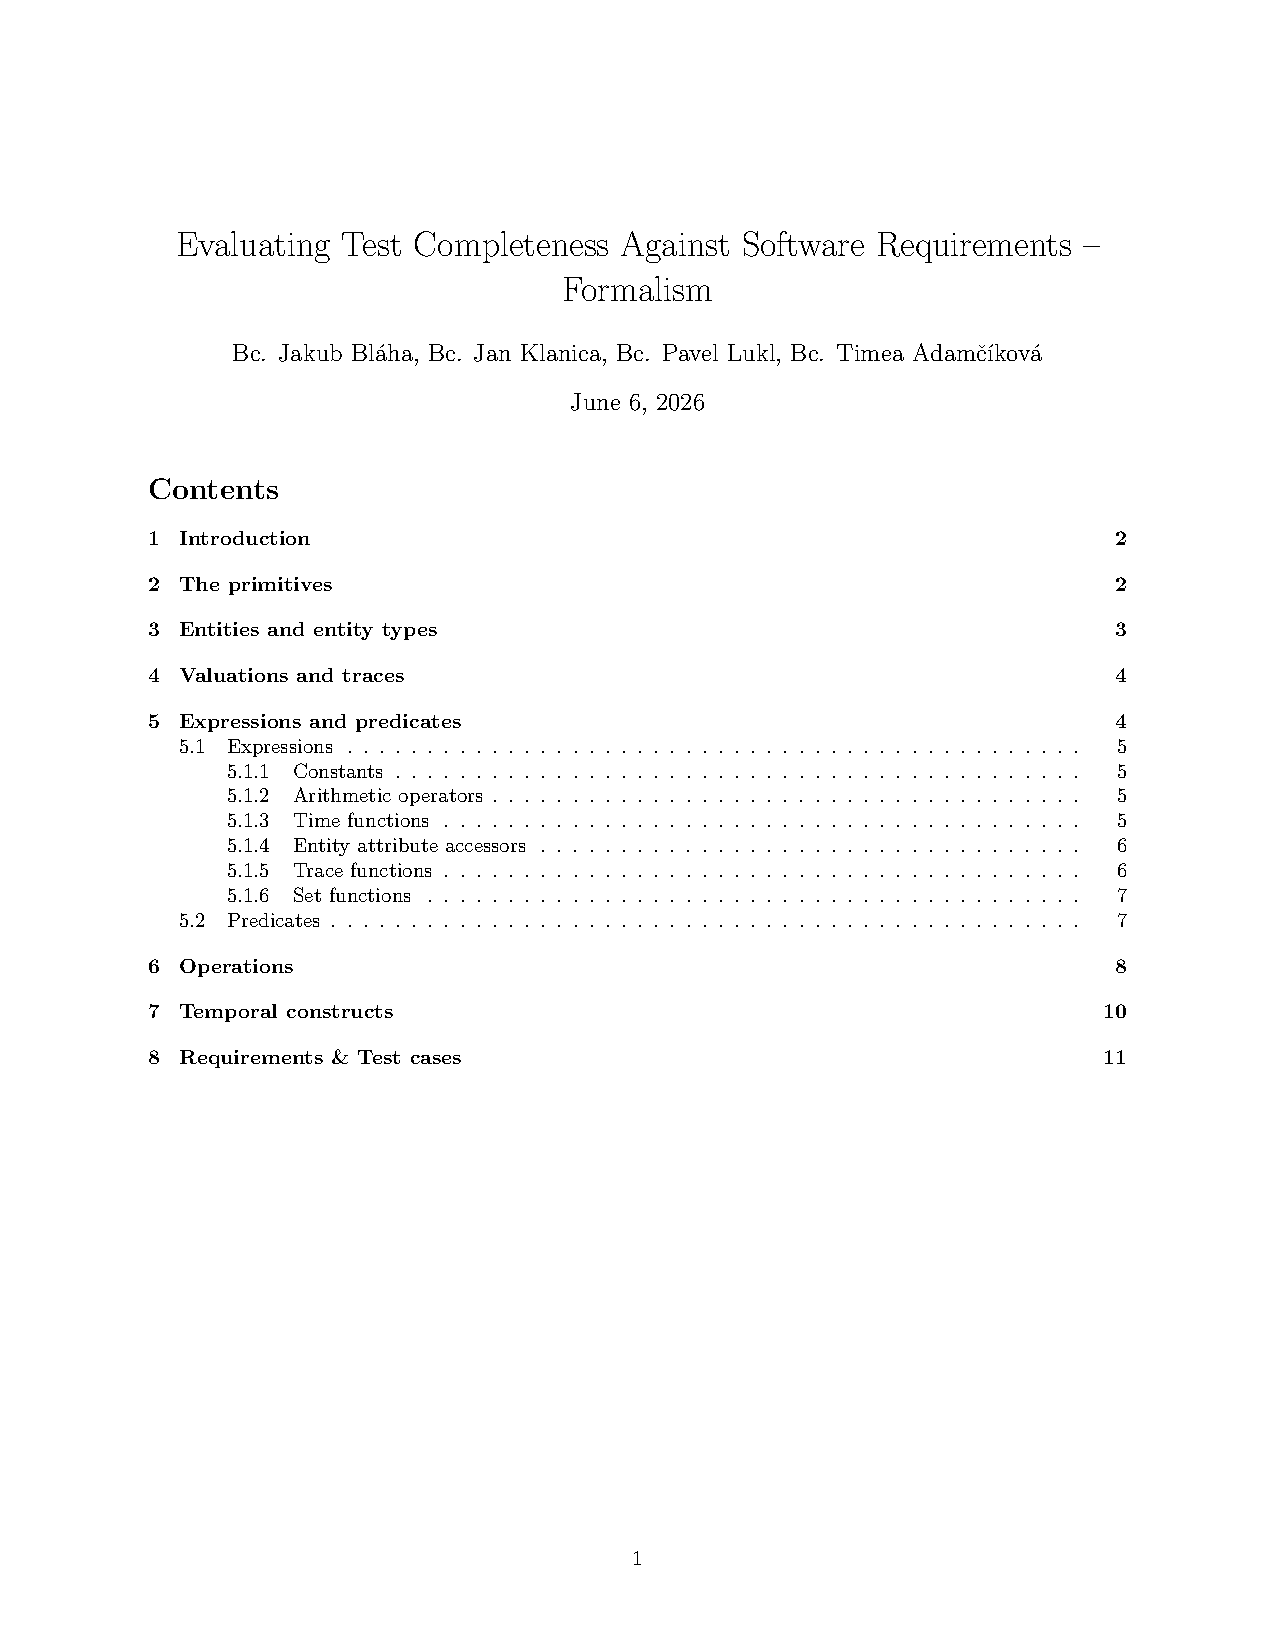
\includepdf[pages=-,pagecommand={}]{pdf/doc}

%--------------------------------------------------------
%--------------------------------------------------------
%--------------------------------------------------------
\end{document}